\documentclass[Main.tex]{subfiles} 


\begin{document}

In this section the basis for the conclusions made in the main sources that are used throughout this paper. The basis containes excerpts from the original source.

\subsection*{Who gets the job referral?, \emph{Beaman, L. \& Magruder, J.} \cite{first}}

\emph{"By interacting initial OP ability with performance pay in column (3), we see that the differential
performance of referrals recruited by high ability OPs is driven by OPs who face performance
pay incentives. Therefore, high ability individuals refer high ability people only when properly
incentivized, suggesting that the networks of high ability OPs are heterogeneous and that high
ability OPs do have the capacity to screen."}\\

This laboratory experiment by Beaman tries to find out who gets job referral by how capable this person was by performing ability test. The OP (original participants) conducted a test and were asked to refer a friend to the "job". This friend also conducted the same test and varying fixed referral and perfomance referral fees were tried out. The above conclusion came out.

\emph{"Thus, while all OPs change their referral choices in response to changing contractual conditions,
only high ability OPs do so in a way which results in higher ability referrals. As the model
emphasized, a variety of possible differences between high and low ability OPs could explain why
performance incentives did not induce low ability OPs to recruit higher ability referrals: they
may not know high ability referrals; they may lack information on the ability of their network
members; or the tradeoff between their network incentives and the performance incentives may
be too large"}\\

Here a conclusion is drawn that low ability OPs did not produce good referrals even with a performance incentive. The authors note a couple of possible reasons.

\subsection*{The relationship between recruiting source and employee success, \emph{Caldwell, D. \& Spivey, W.} \cite{second}}

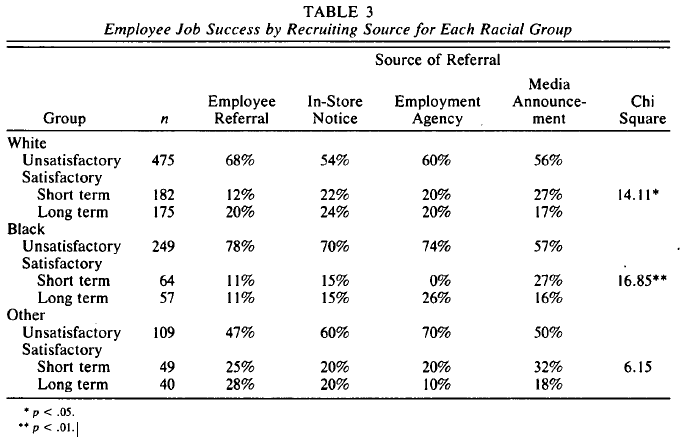
\includegraphics[width=\textwidth]{table3} \\

\emph{"First, while employee referral was relatively
less effective in recruiting satisfactory employees, a disproportionate
number of those were long term."} \\

This study was performed on 1400 store clerks which exhebit an extremely high turnover. After 3 years none of the clerks were still employed at the company. The observation made above is therefore of importance. Employee referral at jobs with high turnover does not lead to better results (or in this case even worse).

\subsection*{The Effect of Workplace Genderand Race Demographic Composition on Hiring Through Employee Referrals, \emph{Taber, M. \& Hendricks, W.} \cite{third}}

\emph{"For example, when an individual comes from a distinct racial
minority in the workplace (0 to 15 percent of the workers are of the same race),that person is almost three times more likely to have been hired through formal sources than employee referral."}\\

This study tries to model the likelihood of a person being referred or employed through formal sources. The argument made is that employees refer to people like themselves as these are available within the network. The above argument shows that other racial minoritities almost do not get referred by the employees if these minorities are not highly present within the firm. Workforce diversity is therefore lowered by employee referral programs.

\subsection*{Recruiting through advertising or employee referrals, \emph{Rafaeli, A. et al.} \cite{fourth}}

\emph{"Two parameters were calculated for each of these recruiting sources: Yield
ratio was the proportion of new hires from the total number of applications
through a given source; cost per new hire was the direct cost of hiring an
applicant, which was computed by dividing the total expenditure per hiring
source by the number of new hires recruited through the source."}\\

The paper tries to model the cost and yield of referral programs.\\

\emph{"As is evident in Table 1, the average cost of hiring through advertising was
significantly higher than hiring through employee referrals (22,652 per new
hire, compared to nothing for hires recruited through referrals). This may
not be surprising given that employee referrals are cost-free, yet the average
cost of recruiting employees through national advertising is a striking
81,000 per hire, confirming the importance of considering cost-per-newhire
in evaluations of recruitment processes. Furthermore, consistent with
our analysis geographically focused ads were far less expensive than
unfocused ads costing 1140 per hire as compared to the striking 81,000 per
hire."}\\

Employee referral leads to significantly cheaper employees compared to formal channels such as advertising. This company did not have a bonus referral program in place and hence no incentives were given to employees to refer.\\

\emph{"Paradoxically the yield ratio of the less costly employee referrals was
significantly greater than that of employment advertising: .133 (109 new
hires out of 821 applicants) as compared to .032 (23 new hires out of 724
applicants). The yield ratio of geographically focused (local) advertising
(.073) was also better than that of geographically unfocused (national)
advertising (.018)."}\\

Employee referral has the highest yield ratio (propertion of new hires) implying that screening done by the employees themselves is effective and leads to better applications than just the advertisement.

\subsection*{Do informal referrals leads to better matches?, \emph{Brown, M. et al.} \cite{fifth}}

\emph{"Our central finding is that referred applicants are indeed more likely to be hired. Among the
set of applicant sources, internet job boards produce the largest number of observed applicants,
and so we employ job boards as the omitted category. Relative to job board applicants, referred
applicants are estimated to be 7.3 percentage points more likely to be interviewed for the position,
and 2.4 percentage points more likely to receive an offer. Conditional on having been interviewed,referred applicants are 13.9 percentage points more likely than job board applicants to receive
offers."}\\

The hypothesis of \emph{referred candidates are more likely to be hired} was comfired and is in line with the results found in the previous subsection.\\

\emph{"The estimated coefficient on referral in the log salary regression, reported in Table 7, indicates
a 2.1 percent starting salary premium for referred workers. The coefficient is significant at the
one percent level. The magnitudes of the referral coefficient estimates in the linear and log salary
regressions are roughly consistent, given mean and median salaries of 102.740 and 97.377, respectively."}\\

Interestingly, referred also receive a higher salary compared to external sources. No clear reason for this in the paper.\\

\emph{"As discussed in Section 3.3, however, current theory of labor market referrals predicts that the
referral effect will dissipate over time, and the salaries of referred and non-referred workers who
remain with the corporation will converge. The log salary estimates reported in Table 7 provide a
test of the referred salary premiums time trajectory.
We find that the referral effect does indeed diminish over time. In all linear tenure specifications
in Table 7, the coefficient on the interaction between the referral indicator and tenure in the
organization, is negative and significant at the one percent level."}\\

This salary advantage diminishes over time however. Theory explains that this is because external market workers will separate over
time and therefore some of the lower quality workers will leave the sample.

\subsection*{Data mining to improve personnel selection and enhance human capital, \emph{Chien, C. \& Chen, L.} \cite{sixth}}

\emph{"In addition, for
the employees of function C, we found that the
employees who had more than one year of previous
work experience and were hired from external channels
would be more likely to quit within three months than those who were hired from internal channels. This finding was supported by domain knowledge
since the employees recruited from internal channels
usually stay longer, since the referrals should have
shared more information about the job and the company.
Thus, this company has adapted this finding
and developed a strategy to raise a campaign for promoting
the referrals by giving cash bonus to successful
hiring."} \\

An interesting argument is made why the tenure of the reffered is longer than external workers is longer. It gives another explanation besides
the usual screening process done by the employee them selves. The paper argues (ungroundedly) that the reffered stay longer because they have
a better idea of the job than the external workers. 

\subsection*{Sources of referral and employee turnover, \emph{Gannon, Martin J.} \cite{seventh}}
This paper compares seven methods or sources that are used to obtain new employees on their influence on employee turnover. The data from 1961 to 1964 is from the New York bank. The data covers a total of 6,390 employees that were hired. 1,934 of those hired left before completing their first year of service with the bank. The results of this research are shown below.\\
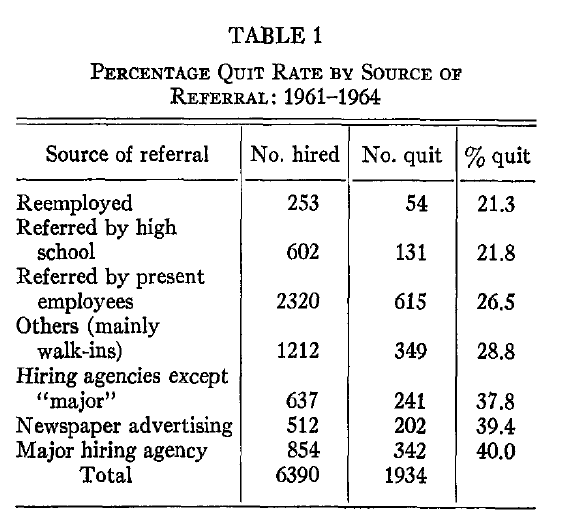
\includegraphics[width=\textwidth]{table1} \\

\emph{Even before an employee approaches a firm
in order to fill out the application form, it is
possible to improve the selection process by
utilizing some sources of referral rather than
others. This study has demonstrated that four
sources of referral are predictive of stable employees,
namely, the reemployment of former
workers of the bank, the hiring of individuals
referred by their high schools, the hiring of
individuals referred by present employees, and
others (primarily walk-ins). However, three
sources of referral are predictive of unstable
employees, namely, the use of hiring agencies
other than the major one, newspaper advertisements,
and the major hiring agency.} \\

The author does not provide an argumentation for why this might be the case.

\subsection*{Relationships between recruiting sources and employee performance, absenteeism, and work attitudes, \emph{Breaugh, James A} \cite{eight}}

This paper examines whether the source by which an individual was recruited is related to employee performance, absenteeism and work attitudes. The sample was composed of 112 research scientists. Most information was gathered by questionaires and information from the personnel records. \\

\emph{With regard to employee performance, the results of the multivariate
and univariate analysis of variances how strong source-of-recruitment differences.
Individuals recruited through college placement offices and, to a
lesser extent, those recruited via the newspaper were inferior in performance
(i.e., quality and dependability) to individuals who made contact
based on their own initiative or a professional journal/convention advertisement.
In terms of absenteeism, another strong source of recruitment
effect was demonstrated. Those recruited through newspaper ads missed
almost twice as many days as did those referred by any of the other
sources. The results of analyses on work attitudes also documented recruiting
source differences. College placement office recruits reported significantly
lower levels of job involvement and satisfaction with supervision
than did employees recruited in other ways.Taken as a whole, these
results demonstrate that college placement offices and newspaper advertisements
were poorer sources of employees than were journal/convention
advertisements and self-initiated contacts.} \\

Journal advertisments and self-initiated contacts did far better than the ones recruited by college placement offices and newspaper advertisements. The argumentation provided for this conclusion is based on the model of Wanous (1978) which states that people that have more complete information about the job will do better than the people that do not have all the information. \\

\emph{Wanous posits that individuals who possess more accurate and
more complete information about a job will be botj more productive and more satisfied than will individuals who have less accurate and less complete information. (...) 
Wanous argues that individuals who have more complete and accurate information
will have a clearer view of what the job entails (role clarity) and this be more likely to perform the job well. (...) Wanous suggests that individuals possessing more complete information will not be likely to consider jobds that do not match their needs.}

\subsection*{The motivations for and outcomes of employee referrals  \emph{Shinnar, Rachel S and Young, Cheri A and Meana, Marta} \cite{ninth}}

This paper describes a model called the Employee Recommenders' Motivation and Outcomes (ERMO) model which describes the motivation of current employees to make a referral. The model is based on Words-Of-Mouth, attitudal advocacy and self-perception theory. The ERMO model predicts that employee recommenders may have different motivations for, but will experience increased organizational normative commitment and job satsifaction from, having referred others to their organizations. \\

\emph{In the context of employee referrals, individuals who have positive job attitudes are likely to engage in Word-Of-Mouth
behavior based on intrinsic motivation. However, the ERMO model also
predicts the outcomes for employee recommenders who do not have possitive work attitudes, but engage in positive WOM as a result of extrinsic
rewards offered by the organization for referrals (such as monetary
inducements).} \\

Based on theory it is believed that the job satisfaction and commitment for the employment are possitively influenced when possitively telling about a job. \\

\emph{Cognitive dissonance theory explains attitude and discrepant behavior while self-perception theory explains
both attitude-congruent and attitude? discrepant behavior. We can
therefore state that attitudinal advocacy theories predict that employees
who 'sell' their organizations to friends or relatives will align their beliefs
with the positive statements they make. } \\

\emph{employees use the referral
conversation as a way to justify their choice of employer.}\\

It is said that when employee referrers tell posstively about their job they will also start to believe in it.
However, the only theory that was supported in the research was the following: \\

\emph{H1a: Engaging in an employment recommendation will lead to an
increase in normative commitment for the recommender immediately after engaging in a referral. }\\

This can be the case because it was an experiment, in real life the referral would take longer which might help.

%\subsection*{Social capital at work: Networks and Employment at a Phone Center, \emph{Fernandez, R.M, Castilla, E.J. , Moore,P} \cite{tenth}}
%\subsection*{Hiring through referrals, \emph{Galenianos, M} \cite{elventh}}
%The aim of this paper is to combine social networks with the equilibrium models that are used to study labor markets. 

\subsection*{The relationship between recruiting source, applicant quality, and hire performance: An analysis by sex, ethnicity, and age, 
\emph{Kirnan, Jean Powell and Farley, John A and Geisinger, Kurt F} \cite{tenth}}

This paper investigated the different recruiting sources and the quality of the employee. 
There are two main theories used in this paper.
\emph{Two major theories have been advanced to explain the predominant
finding that informal sources provide superior employees: (1) the prescreening hypothesis and (2) the realistic job information hypothesis. The
prescreening hypothesis states that differences in new hire success across
recruiting sources can be traced to corresponding differences in the quality
of applicants across recruiting sources (...) The assumption is that applicants referred by current employees (the predominant informal recruiting source) are prescreened by these
employees. As "screeners," current employees have the benefit of knowing
both the job and the individual. Armed with this information, they are able
to refer those applicants who are well qualified for the job}\\

The conclusion of this article is the same as most of the others, the informal sources lead to better employees than the formal resources.\\

\emph{Referrals by agent, district manager, sales manager,
and those individuals whose application was self-initiated had significantly
higher BQ scores than applicants from the other sources. The sources
of mutual acquaintance and some other way were next, followed in order
by newspaper advertisements, employment agency and school placement.}\\

\emph{Referring to these figures, it is clear that the informal sources are
responsible for a proportionately greater number of hires }\\

There were however, some differences between sex, age and ethnic background. \\

\emph{When significant differences were apparent, they were in
the direction of males, older applicants and non-minorities scoring higher
than their female, younger, and ethnic minority counterpart}\\

\emph{The results indicated that females and blacks
used a proportionately greater number of formal recruiting sources than did
their male and non-minority counterparts.}\\

This might be explained by the following:\\
\emph{The logic was that if the current workforce were
predominantly male and non-minority, then current employees would most\\
often refer applicants like themselves (e.g., other white males).}

The differences indicate that a company still should use the formal advertisments to have a diverse team. 

\emph{Although
the informal sources produced the best quality applicants for all groups (the
best males, best females, etc.) one cannot issue a blanket policy recommending its exclusive usage. Given the disproportionately large number
of female and black applicants utilizing newspaper ads in this study, such
a move would result in a reduction in the number of female and black
applicants.}\\


\subsection*{Recruiting methods and turnover, \emph{Keaveny, Timothy J and Allen, Robert E} \cite{eleventh}}
This paper finds a difference between business administration graduates and engineering graduates in turnover.\\

\emph{Among business administration graduates in the sample, 
some support is observed for the hypothesis that personal referrals 
are associated with lower turnover. Those leaving their initial 
employer were less likely to have used personal references than 
either formal methods or direct applications. However, support for 
the hypothesis was not found when the engineering subsample was 
examined.}\\

\emph{There are several possible explanations for the association 
between turnover and recruiting method characterizing the 
business subsample. Individuals using alternative job sources may 
differ with respect to their inherent abilities. It is possible that 
higher turnover among those using formal methods, primarily 
college placement offices in this sample, occurs because they are 
more qualified than their counterparts using other job sources. 
As a result, more employment opportunities might be available 
to them. They might also be more aggressive, have higher needs for 
achievement, or make greater efforts to seek out other job oppor- 
tunities. Alternatively, the lower turnover among members of the 
business subsample using personal referrals could be a function 
of favorable interpersonal relations. Perhaps peer group relations 
and superior-subordinate relations are better when one uses this 
method to obtain employment. Also, it is possible that an 
individual obtaining a job this way feels an obligation to stay with 
a job longer than is the case with other recruiting methods.}\\ 

\emph{Within the engineering subsample, the proportion changing 
employers was approximately the same for individuals using 
personal referrals and formal methods. However, those using direct 
applications were less likely to change employers than those 
utilizing the other job sources. It is possible that individuals 
utilizing direct applications have made a greater investment in 
time and effort to obtain their initial positions. As a result, they 
may be less likely to leave that employer.}\\

Interesting is also, this paper finds that personal referrals lead to lower level jobs\\

\emph{The association between recruiting method and job level 
was significant for both groups, but in the direction opposite 
than predicted. Formal methods were associated with higher level 
jobs and personal referrals with lower level jobs.}\\

The following explanation is given for this findings:\\

\emph{. It is quite likely that the effective use of 
informal job sources is contigent upon a network of contacts 
which can transmit labor market information to the job seeker. 
The two-year college graduates participating in this study may 
not have a system of personal contacts as well developed as 
that characterizing the older, more experienced respondents 
to the other studies. As a result, the two-year college graduates 
may receive relatively poorer jobs through their personal contacts.}\\

Or the fact that people are not sure enough to change their job:\\

\emph{The hypotheses, however, ignored one significant 
aspect of the turnover decision. Not only is turnover influenced 
by the perceived desirability of a job change, it is also determined 
by the perceived ease of movement (6). It is quite possible that the two-year graduates in the less attractive jobs wanted to change 
employers (the essence of the hypotheses), but did not think it 
was feasible for them to do so. }\\


\subsection*{Social Networks and Labor-Market Outcomes, \emph{Montgomery, J.D.} \cite{twelveth}}
The author of this paper developed a model which explicitely incorporates a simple social structure.
The model explains why workers that have good connections might fare better and why firms hiring through referral might earn higher profits.\\

\emph{(...)workers with no social ties to high-ability workers are forced to find employment through the market, earning a relatively low wage due to the lemons effect} \\
The lemons effect means competition between firms drives the market wage below the average productivity of the population.
This is the main conclusion and explanation I could find in the paper.


\end{document}